 \documentclass[12pt,a4paper,titlepage]{article}
\usepackage[utf8]{inputenc}
\usepackage[finnish]{babel}
\usepackage{setspace}
\usepackage{subcaption}
\usepackage{fancyhdr}
\usepackage[top=1in, bottom=1in, left=1in, right=1in]{geometry}
\usepackage{float}
\usepackage{pdfpages}
\usepackage{enumitem}
\usepackage{tabularx}

\usepackage{hyperref}
\hypersetup{pdfborder={0 0 0}}
\onehalfspacing
\cfoot{}
\rhead{\thepage}
\lhead{\leftmark}

\title{Tsoha\\ Kurssikysely \vspace{0.5em}}
\author{Anni Järvenpää}
\date{\today}

\begin{document}
\maketitle

% Sisällysluettelo
\newpage
\tableofcontents
\thispagestyle{empty}
\newpage
\setcounter{page}{1}
\parskip=1em \advance\parskip by 0pt plus 2pt
\pagestyle{fancy}
\cfoot{\thepage}

%%%%%%%%%%%%%%% Oleellinen sisältö alkaa%%%%%%%%%%%%%%%
\section{Johdanto}
Työn tavoitteena on toteuttaa kurssikyselyjärjestelmä, jonka avulla opiskelijoilta voidaan kerätä palautetta kursseista. Kurssin luennoitsija luo luennoimalleen kurssille kyselyn ja lisää kyselyyn kysymykset. Kysymyksiä on myös mahdollista muokata tai poistaa kyselyn avaamiseen asti. Kyselyn oltua avoinna vastattavaksi, voi luennoitsija sulkea kyselyn, jolloin uusia vastauksia ei voi enää antaa. Hallintohenkilöt luovat kurssit ja asettavat niiden tiedot (opettaja, kotisivu yms). Opiskelijat vastaavat kyselyihin sellaisista kursseista, jolla opiskelija itse on osallistujana.

\section{Yleiskuva järjestelmästä}
Järjestelmää käyttävät opiskelijat, opettajat ja hallintohenkilöt. Näistä kaikki voivat kirjautua järjestelmään. Kirjauduttuaan opiskelijat näkevät kyselyt kursseista, joilla ovat osallistujina, opettajat kyselyt kursseista, joilla ovat opettajina. Mikäli jollakin kurssilla ei vielä ole kyselyä, näytetään sen opettajalle kurssin tiedot ja annetaan mahdollisuus lisätä kurssille kyesly. Hallintohenkilöt näkevät listan kaikista olemassaolevista kursseista. Käyttö\-tapaus\-kaavio on nähtävillä kuvassa \ref{fig:kayttotapauskaavio} ja käyttötapaukset on eritelty alla.

\begin{figure}
   \centering
   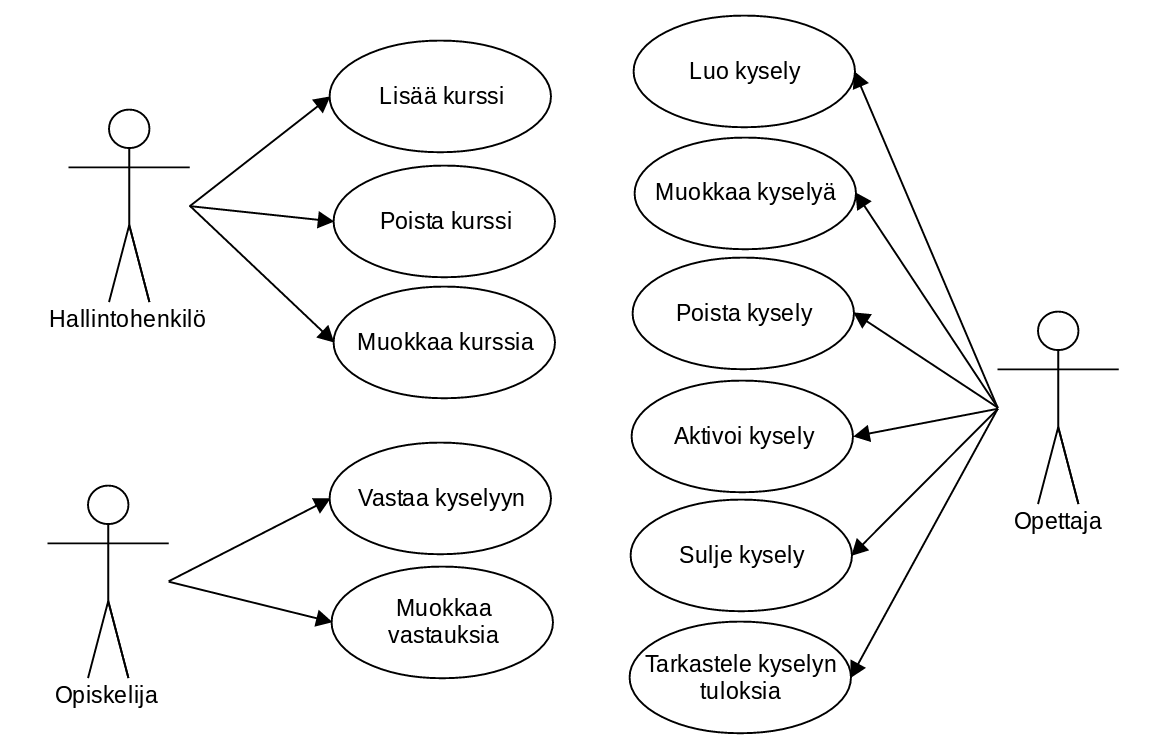
\includegraphics[width=\textwidth]{kuvat/kayttotapauskaavio.png}
   \caption{Järjestelmän käyttötapauskaavio. Kaavioon merkittyjen käyttötapausten lisäksi jokainen järjestelmän käyttäjäryhmä pystyy kirjautumaan järjestelmään.}\label{fig:kayttotapauskaavio}
\end{figure}

\begin{description}[style=nextline]
    \item[Kirjautuminen] Kaikki käyttäjäryhmät voivat kirjautua palveluun ja palvelun käyttäminen alkaa aina kirjautumisella.
    \item[Kyselyiden selaaminen] Kirjautumisen jälkeen opiskelija ja opettaja siirtyvät selaamaan kyselyitä. Näytettävien kyselyjen määrä ja kyselyistä näytettävät tiedot riippuvat käyttäjästä.
    \item[Kyselyn tulosten tarkasteleminen] Päättyneiden kyselyiden tuloksia voi tarkastella. Tällöin näytetään kunkin kysymyksen vastausjakauma.
    \item[Kyselyn luominen] Opettaja pystyy luomaan opettamalleen kurssille kyselyn. Tällöin avataan tyhjä kysely muokkaustilassa.
    \item[Kyselyn muokkaaminen] Opettaja voi muokata oman kyselynsä kysymyksiä. Tällöin hänelle näytetään lista nykyisistä kysymyksistä ja annetaan mahdollisuus poistaa niitä tai siirtyä luomaan uusia tai muokkaamaan vanhoja. Kyselyn muokkaaminen ei onnistu enää kun kysely on avattu opiskelijoille.
    \item[Kyselyn tilan muuttaminen] Kurssin opettaja voi muuttaa kyselyn tilan luonnoksesta käynnissä olevaksi, jolloin opiskelijat voivat vastata kyselyyn, tai käynnissä olevasta päättyneeksi, jolloin kyselyyn ei voi enää vastata mutta kyselyn opettaja voi tarkastella kyselyn tuloksia.
    \item[Kysymyksen lisääminen] Kysymystä lisättäessä opettaja voi antaa kysymyksen. Kysymykset on muotoiltava niin, että niihin voidaan vastata asteikolla 1-5 tai EOS.
    \item[Kysymyksen muokkaaminen] Kysymyksen muokkaaminen toimii vastaavasti kuin kysymyksen lisääminen, mutta oletusarvoina käytetään kysymyksen nykytilaa.
    \item[Kurssin lisääminen] Laitoksen hallintohenkilöt voivat lisätä kursseja. Tällöin kurssista annetaan sen nimi, opettaja tai opettajat, kurssin alkamis- ja päättymispäivät ja mahdollisesti linkki kurssin kotisivulle.
    \item[Kurssin muokkaaminen] Laitoksen hallintohenkilöt voivat muokata kurssien tietoja niistä kursseista, joilla ei ole kyselyitä, jotka olisivat olleet vastattavissa.
    \item[Kurssin poistaminen] Laitoksen hallintohenkilöt voivat poistaa kursseja. Tällöin myös kurssiin liittyvät kyselyt, kysymykset ja vastaukset poistuvat.
\end{description}

\section{Järjestelmän tietosisältö}
\begin{figure}
   \centering
   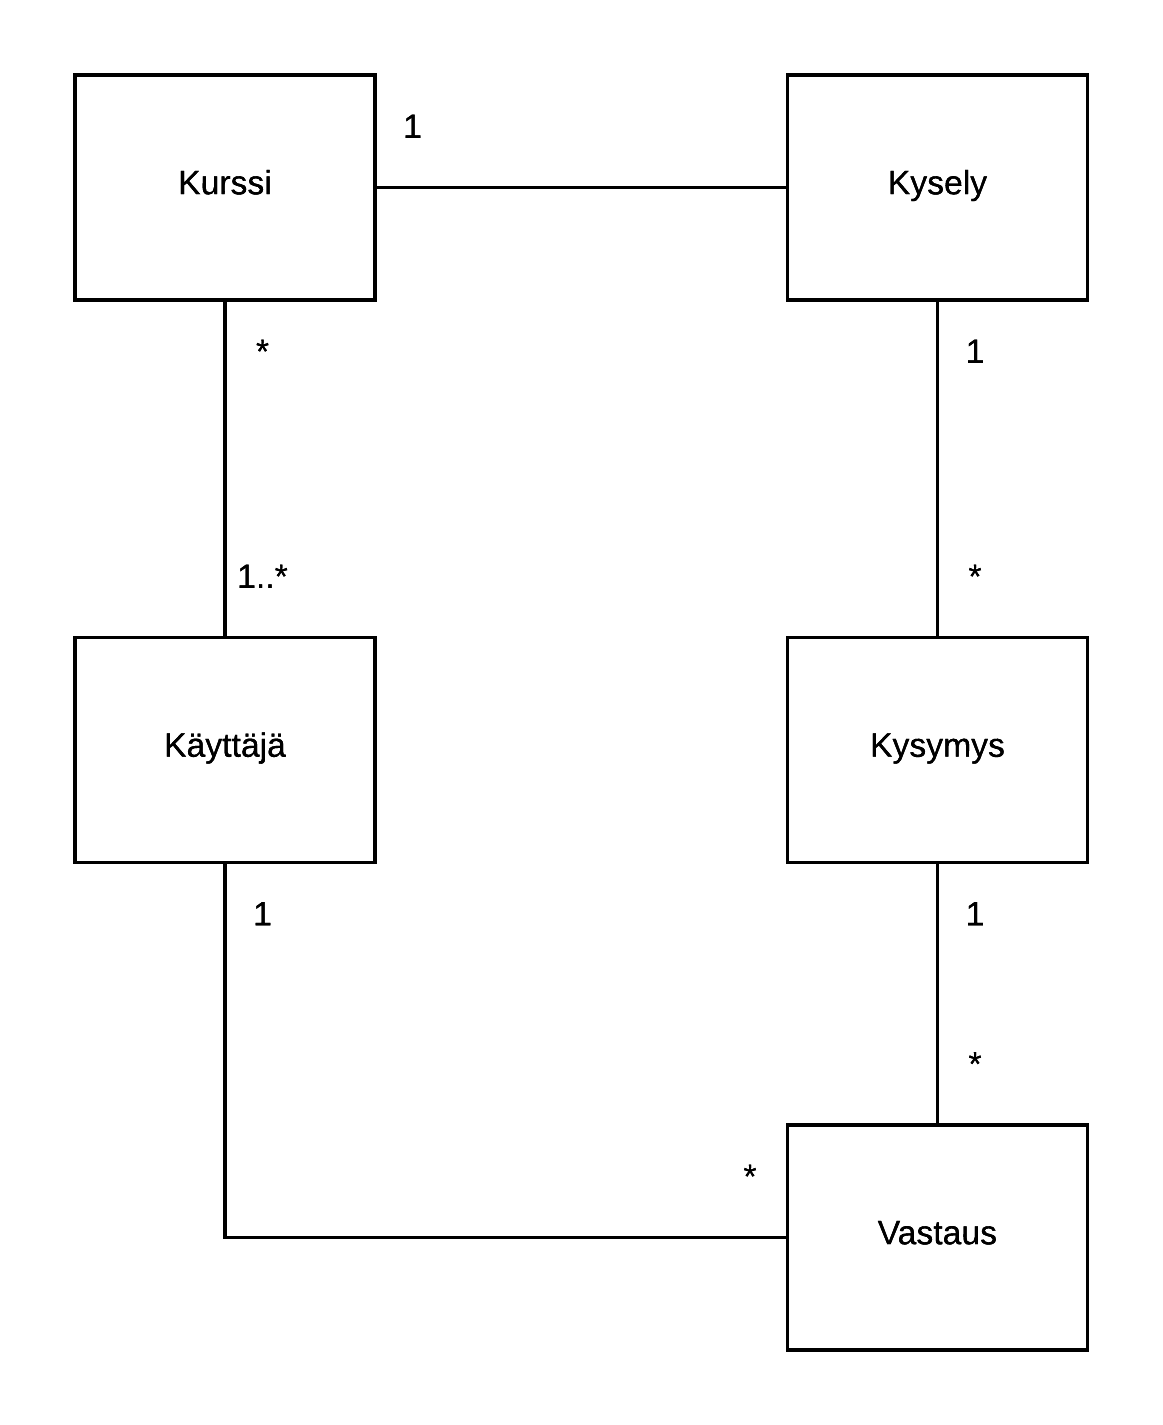
\includegraphics[width=0.6\textwidth]{kuvat/kasitekaavio.png}
   \caption{Käsitekaavio järjestelmään tallennettavasta tiedosta}\label{fig:kasitekaavio}
\end{figure}

Järjestelmän tietosisältö on esitetty kuvassa \ref{fig:kasitekaavio}. Tarkemmat esittelyt kustakin käsitekaavion tietokohteesta ovat nähtävissä alla sekä taulukoissa \ref{tietokohde_ensimmainen}--\ref{tietokohde_viimeinen}.

Kukin järjestelmän käyttäjä on joko hallintohenkilö tai muu henkilö (opettaja ja/tai opiskelija). Lisäksi käyttäjästä tallennetaan käyttäjätunnuksena toimiva sähköpostiosoite sekä hashattu salasana ja suola.

Kysely edustaa tietyn kurssin palautekyselyä. Kyselyn tilat on tallennettu erilliseen tauluun, jotta tilojen nimitykset on helppo pitää konsistentteina muutoksista huolimatta ja tilojen arvojoukko on helppo tarkastaa. Kutakin kurssia kohden on yksi korkeintaan yksi kysely ja kukin kysely voi koostua mielivaltaisestsa määrästä kysymyksiä. Kukin kysymys kuuluu yhteen kyselyyn. Kutakin kysymystä kohden voi olla mielivaltainen määrä vastauksia, kuitenkin korkeintaan yhtä paljon kuin kurssilla on opiskelijoita. Vastaus-tauluun tallennetaan vastauksen antaneen opiskelijan ID, kyseisen kysymyksen ID sekä opiskelijan antama vastaus. Vastaus tallennetaan lukuna 0-5 joista 1-5 edustavat varsinaisia numeerisia vastauksia ja 0 vaihtoehtoa "en osaa tai halua vastata".


\begin{table}[h!]
\caption{Käyttäjä} \label{tietokohde_ensimmainen}
\begin{tabularx}{\textwidth}{ | l X X |}
  \hline
  Attribuutti & Arvojoukko & Kuvailu \\
  \hline
  sähköposti & Merkkijono, korkeintaan 256 merkkiä & Käyttäjän sähköpostiosoite. Tätä käytetään viestinnän lisäksi kirjautumiseen. \\
  salasanaHash & Merkkijono, käytetystä salausalgoritmista riippuva maksimipituus tarkentuu myöhemmin. Tällä hetkellä käytössä 256. & Käyttäjän salasana suolattuna ja hashattynä\\
  suola & Merkkijono, käytetystä salausalgoritmista riippuva maksimipituus tarkentuu myöhemmin. Tällä hetkellä käytössä 16. & Käyttäjän salasanaa hashattaessa käytetty suola \\
  hallintohenkilö & Totuusarvo & True jos käyttäjä on hallintohenkilö, muuten false. \\
  \hline
\end{tabularx}
\end{table}

\begin{table}[h!]
\caption{Kurssi}
\begin{tabularx}{\textwidth}{ |  l X X  |}
  \hline
  Attribuutti & Arvojoukko & Kuvailu \\
  \hline
  Nimi & Merkkijono, korkeintaan 150 merkkiä & Kurssin nimi, esimerkiksi "Aineopintojen harjoitustyö: Tietokantasovellus (periodi II)" \\
  Kurssikoodi & Kokonaisluku & Kurssin koodi \\
  Kotisivu & Merkkijono, korkeintaan 500 merkkiä & Kurssin kotisivun URL. NULL, jos kurssilla ei ole kotisivua. \\
  Alkamispäivä & Date, ei päättymispäivää myöhemmin & Kurssin alkamispäivä \\
  Päättymispäivä & Date, ei alkamispäivää aiemmin & Kurssin päättymispäivä \\
  \hline
\end{tabularx}
\end{table}

\begin{table}[h!]
\caption{Kysely}
\begin{tabularx}{\textwidth}{ |  l X X  |}
  \hline
  Attribuutti & Arvojoukko & Kuvailu \\
  \hline
  Kurssi & Viite kurssiin & Kurssi, johon kysely kuuluu. \\
  Status & Viite tila-tauluun & Kurssin tämänhetkinen tila. \\
  \hline
\end{tabularx}
\end{table}

\begin{table}[h!]
\caption{Kysymys}
\begin{tabularx}{\textwidth}{ |  l X X  |}
  \hline
  Attribuutti & Arvojoukko & Kuvailu \\
  \hline
  KyselyID & Viite kyselyyn tai NULL & Viite kyselyyn, mikäli kyseessä on tiettyyn kyselyyn liittyvä kysymys \\
  Teksti & Merkkijono, korkeintaan 500 merkkiä & Opiskelijalle näytettävä kysymys \\
  \hline
\end{tabularx}
\end{table}

\begin{table}[h!]
\caption{Vastaus}
\begin{tabularx}{\textwidth}{ |  l X X  |}
  \hline
  Attribuutti & Arvojoukko & Kuvailu \\
  \hline
  OpiskelijaID & Viite opiskelijaan & Vastauksen antanut opiskelija \\
  KysymysID & Viite kysymykseen & Kysymys, johon vastaus liittyy \\
  Vastaus & kokonaisluku & Opiskelijan vastaus. 0 tarkoittaa vastausta "En osaa tai halua vastata", luvut 1-5 numeerisia vastauksia. \\
  \hline
\end{tabularx}
\end{table}

\begin{table}[h!]
\caption{Tila} \label{tietokohde_viimeinen}
\begin{tabularx}{\textwidth}{ |  l X X  |}
  \hline
  Attribuutti & Arvojoukko & Kuvailu \\
  \hline
  Nimi & Merkkijono, korkeintaan 150 merkkiä & Teksti, joka kuvaa kyselyn tilaa\\
  \hline
\end{tabularx}
\end{table}

\section{Relaatiotietokantakaavio}
Käsitekaavion perusteella rakennettu relaatiokaavio on nähtävissä kuvassa \ref{fig:relaatiokaavio}. Siihen on lisätty tarvittavat liitostaulut ja siinä ovat nähtävissä myös taulujen primary keyt (osalla erikseen lisätty ID, jota ei ole tarpeettomana sisällytetty käsitekaavion yhteydessä esitettyihin taulukoihin). Lisäksi kuvassa on esitetty taulujen foreign keyt.

\begin{figure}
   \centering
   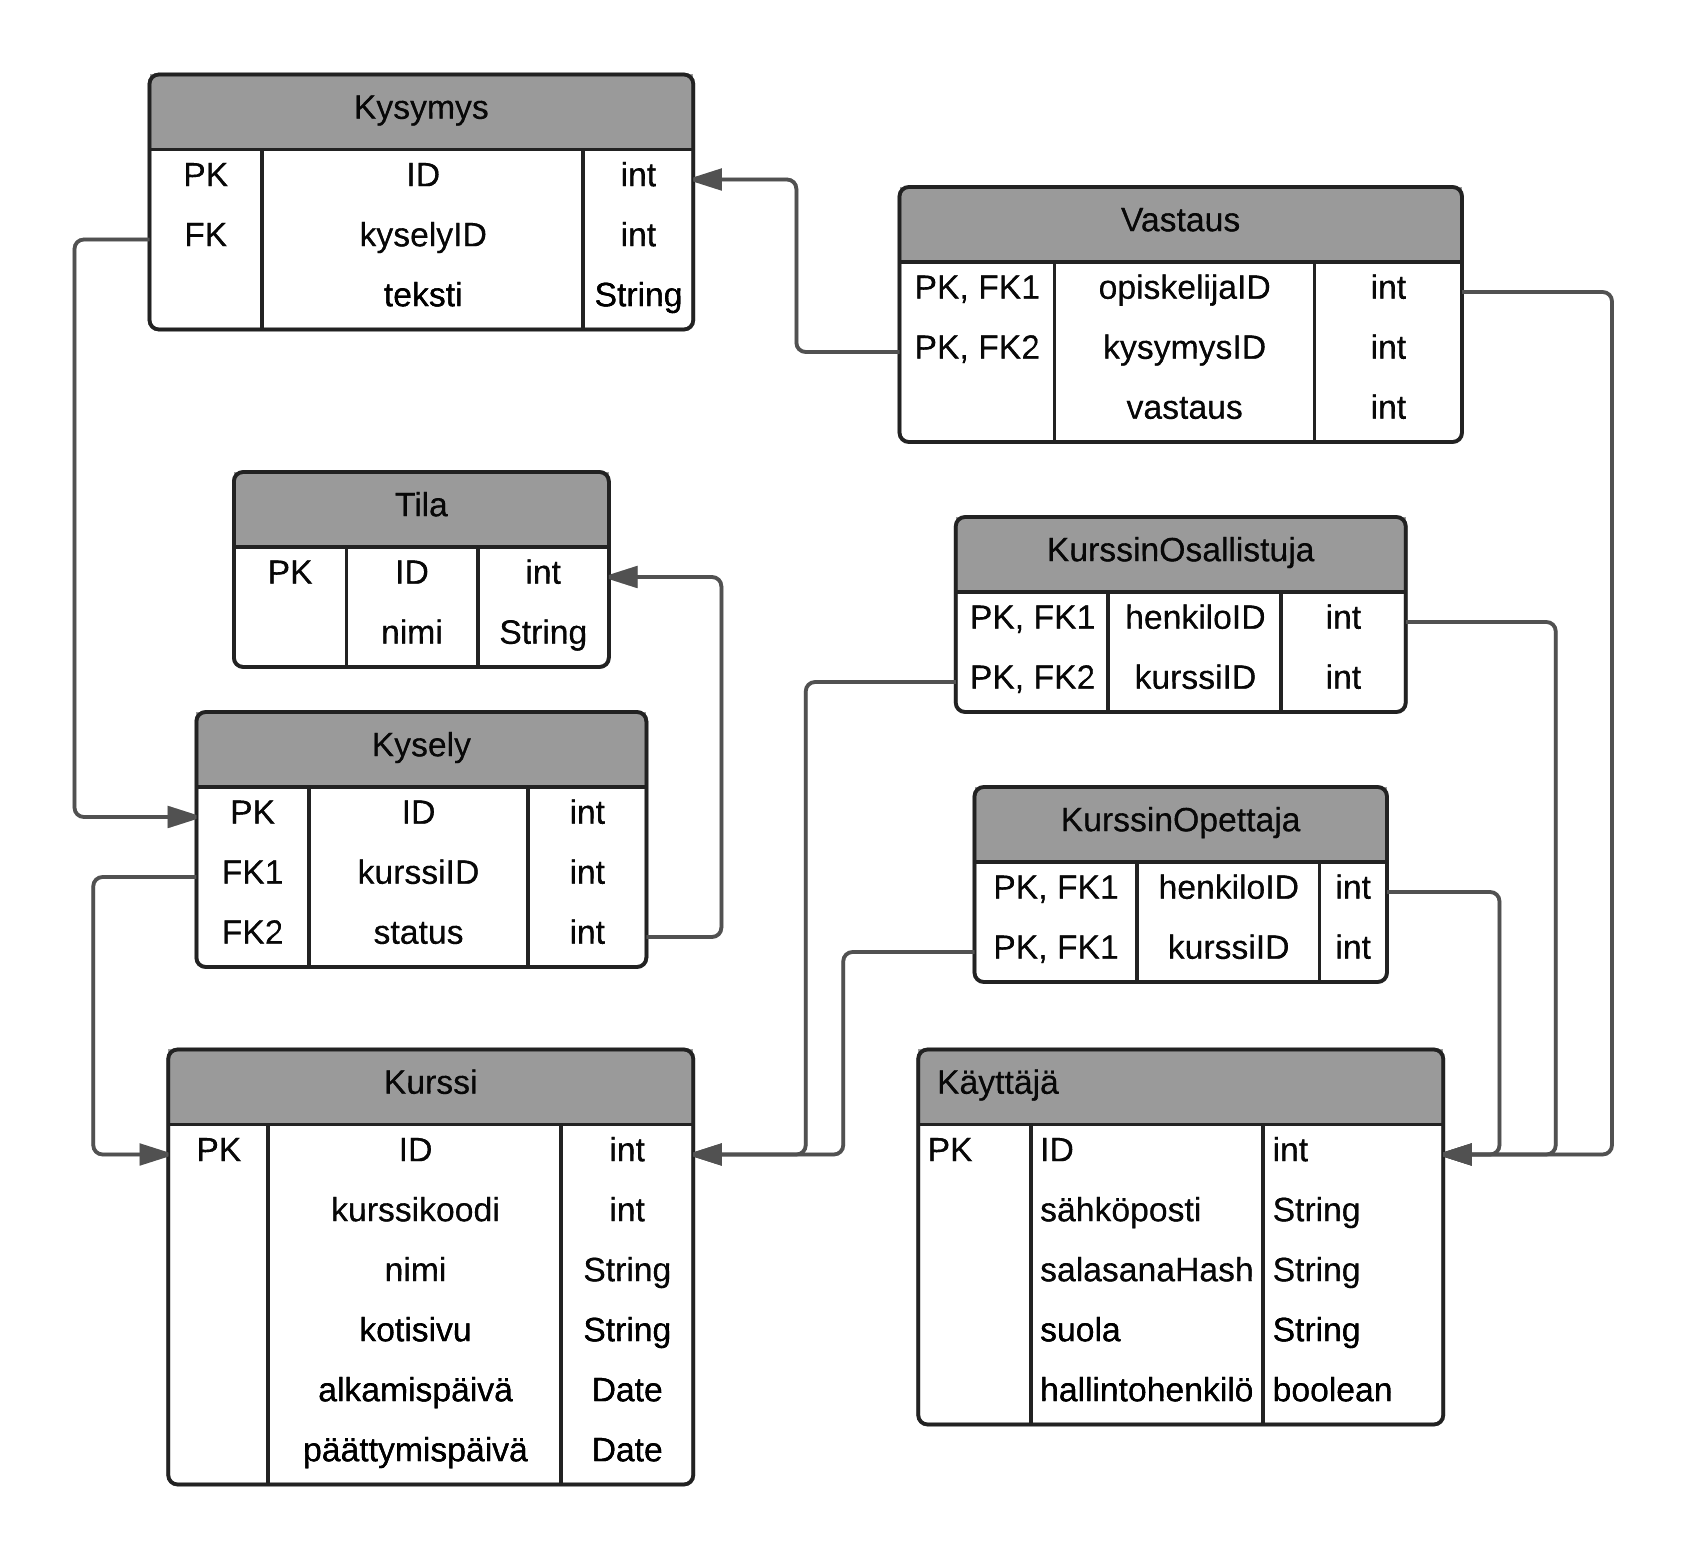
\includegraphics[width=\textwidth]{kuvat/relaatiokaavio-pysty.png}
   \caption{Järjestelmän relaatiokaavio}\label{fig:relaatiokaavio}
\end{figure}

\section{Järjestelmän yleisrakenne}
Tietokantasovellus noudattaa MVC-mallia, jossa kontrollerit, näkymät ja mallit on eroteltu toisistaan. Nämä sijaitsevat hakemistoissa controllers, views ja models. Apukirjastot löytyvät hakemistosta lib. Tiedostot on nimetty pienin kirjaimin, muuttujat ja funktiot camelCasella.

Järjestelmä tallentaa istunnon tietoihin käyttäjän ID:n, jonka perusteella valitaan käyttäjälle näytettävät kurssit. Lisäksi tallennetaan tieto siitä, onko käyttäjä hallintohenkilö, jolloin on helppoa näyttää hallintohenkilöille kurssilistaus ja opettajille ja opiskelijoille kyselylistaus.

\section{Käyttöliittymä ja järjestelmän komponentit}
Järjestelmän näkymien väliset yhteydet ovat nähtävissä kaaviossa \ref{fig:komponentit}. Kaikki muut näkymät paitsi kirjautumissivu edellyttävät sisäänkirjautumista. Tämän jälkeen käyttäjäryhmän perusteella päätetään, näytetäänkö käyttäjälle kysely- vai kurssilistaus. Jokaisesta näkymästä on lisäksi mahdollista siirtyä takaisin kirjautumissivulle käyttäen uloskirjautumisnappulaa, mutta tätä ei ole sotkuisuuden välttämiseksi piirretty näkyviin kaavioon.

\begin{figure}
   \centering
   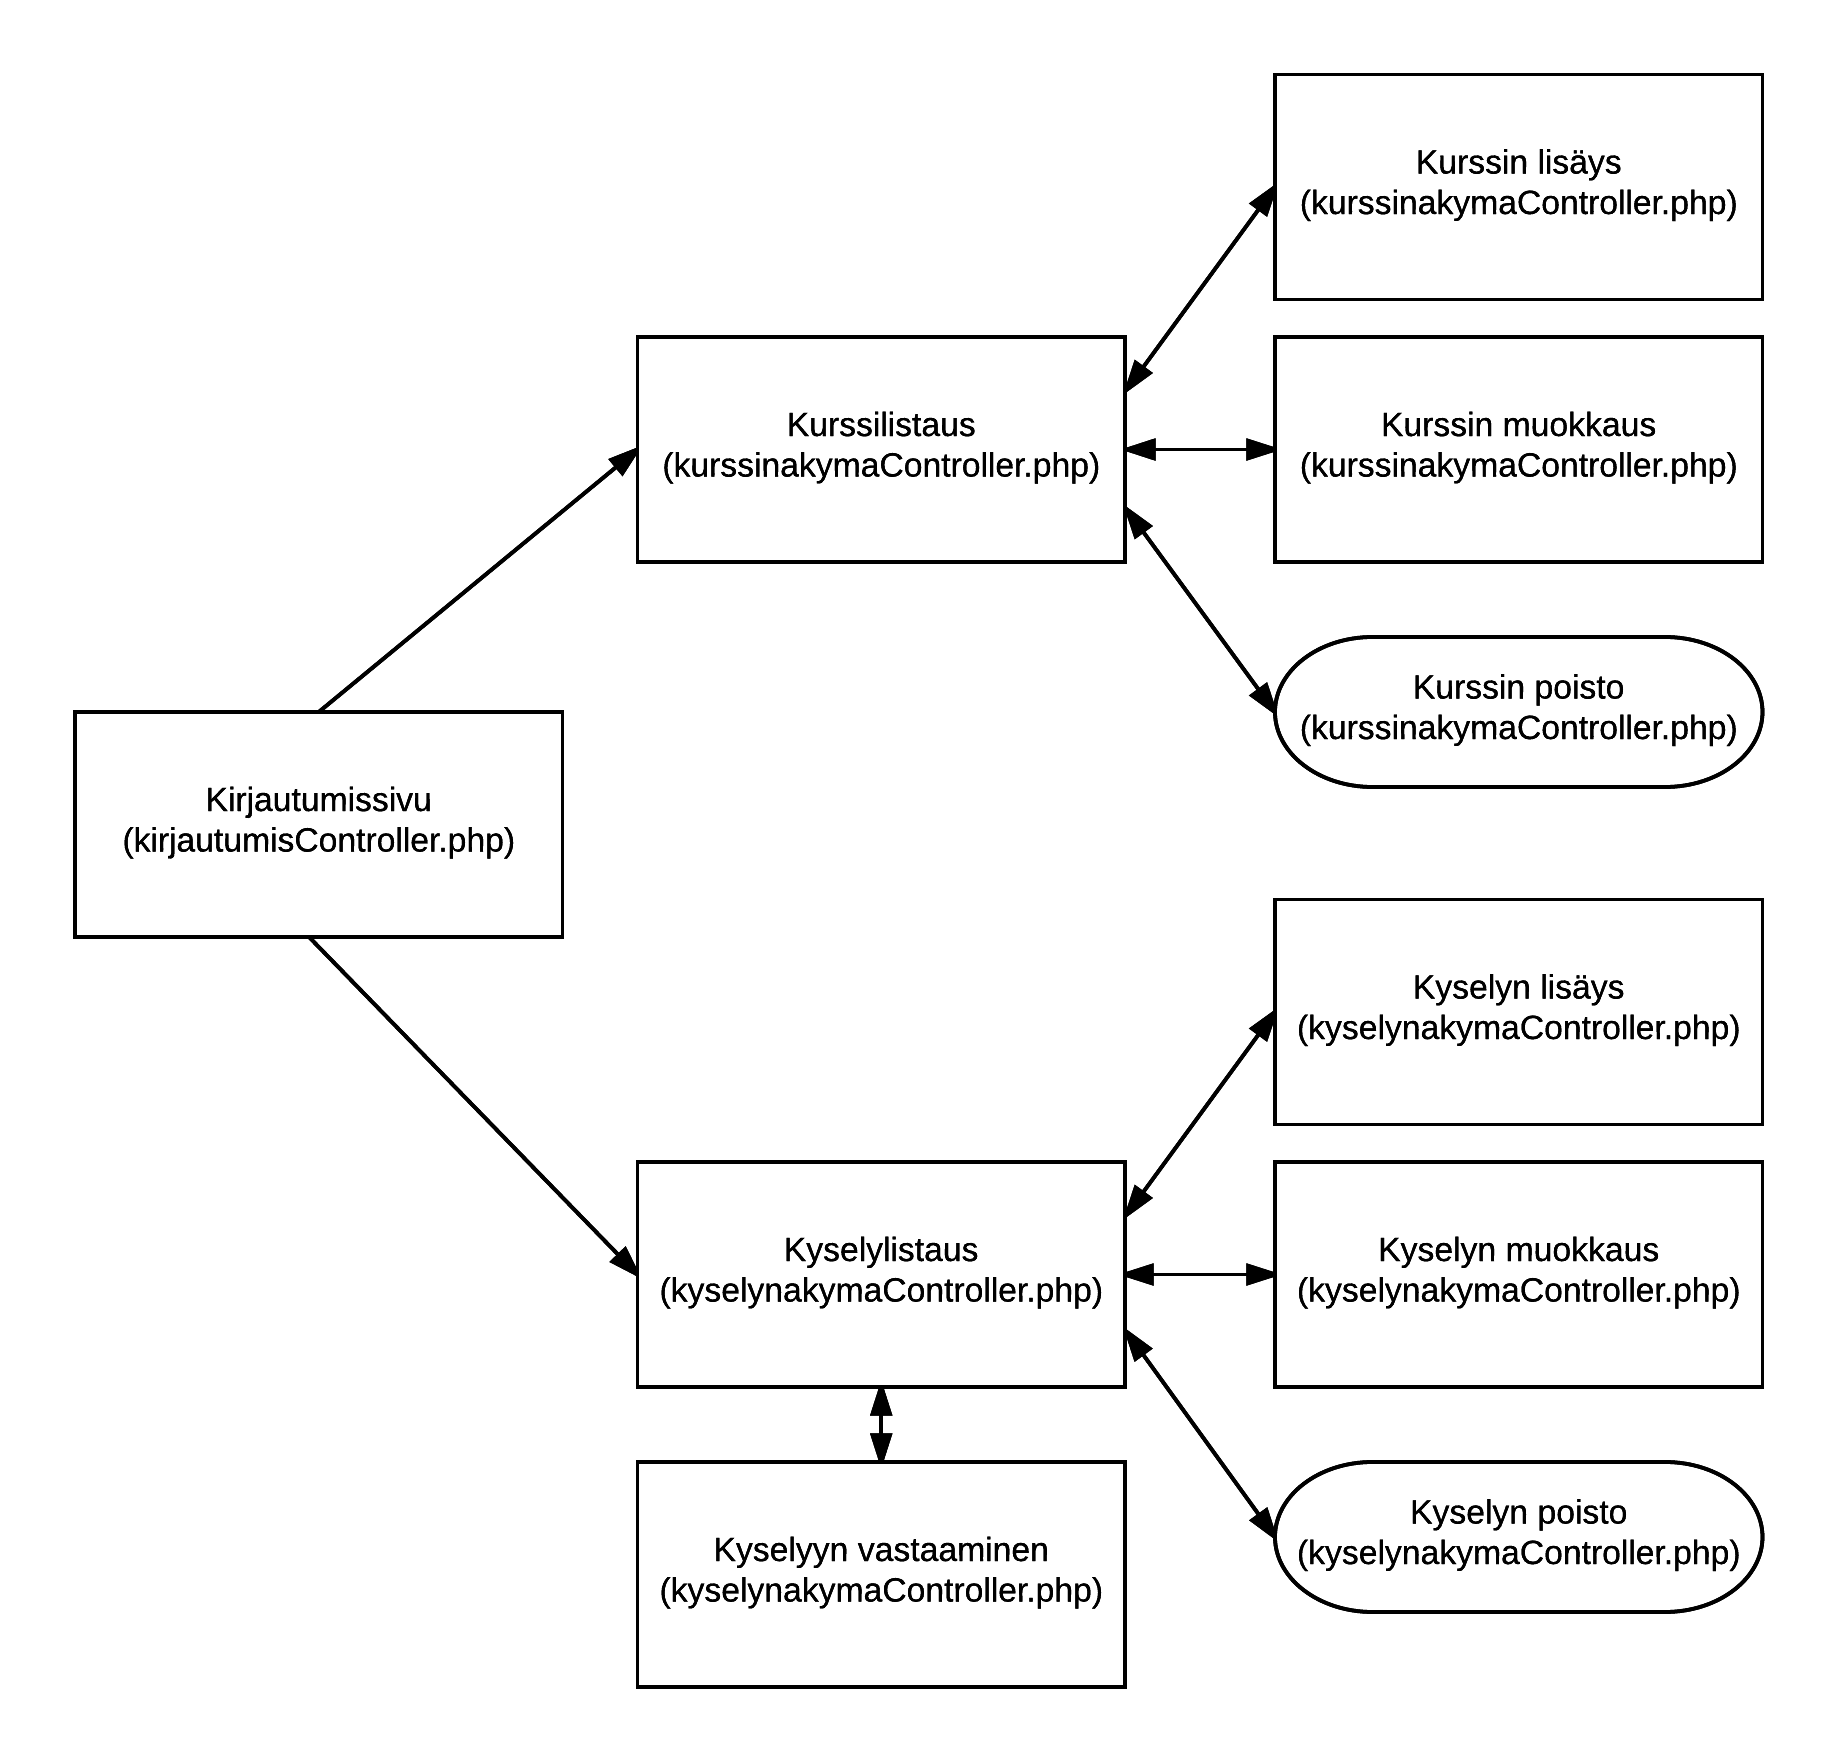
\includegraphics[width=\textwidth]{kuvat/komponenttirakenne.png}
   \caption{Järjestelmän relaatiokaavio}\label{fig:komponentit}
\end{figure}

\section{Asennustiedot}
Muiden on mahdollista asentaa sovellus users-palvelimelle kopioimalla sen tiedostot (github-repositorio \url{https://github.com/aajarven/Tsoha-Bootstrap}) kohdepalvelimelle sopivaan hakemistoon ja tämän jälkeen muokkaamalla projektin config-kansiossa olevassa envi\-ronment.sh-tiedostossa määritellyt username ja project folder sopiviksi. Muulle kuin usersille asennettaessa täytyy myös muita skriptejä muokata jonkin verran, muun muassa deploy.sh -skriptin tulee tietää palvelimen osoite.


\section{Käynnistys- ja käyttöohje}
Sovellus on käytettävissä osoitteessa \url{http://aajarven.users.cs.helsinki.fi/tsoha/}. Järjestelmää pääsee käyttämään opettajana kirjautumalla sisään sähköpostiosoitteella "opettaja.tahtinen@helsinki.fi", hallintohenkilönäkymään sähköpostiosoitteella "hallintokaytava@helsinki.fi ja opiskelijana "oppilas.hononen@helsinki.fi". Jokaisessa salasanana on "salasana". 

\section{Testaus ja jatkokehitysideat}
Järjestelmää on testattu käyttämällä järjestelmän toimintoja monipuolisesti aina merkittävien muutosten tekemisen jälkeen. Automatisoituja yksikkötestejä ei ole. Testauksessa ohjelman lopullisesta versiosta ei löytynyt bugeja.

Järjestelmä toimii muuten menettelevästi, mutta olisi mielekästä mikäli opettaja voisi saada kurssinsa palautteesta jonkinlaisen yhteenvedon, joka voisi sisältää esimerkiksi eri kysymysten vastausten keski- ja hajontalukuja. Lisäksi olisi hauskaa toteuttaa alkuperäisessä tehtävänannossa mainittu organisaatiohierarkia, jossa kaikilla esimerkiksi laitoksen kursseilla on yhteisiä kysymyksiä, joiden vastauksia kyseisen organisaatiotason hallintohenkilöt pääsevät tarkastelemaan.

Ohjelman suurimpana puutteena pidän kuitenkin sitä, ettei nettikäyttöliittymä tarjoa mahdollisuutta lisätä opiskelijoita kurssille, vaan tämä on tehtävä suoraan tietokantaan. Mikäli aikaa olisi enemmän, olisi tämä ensimmäinen ominaisuus jonka toteuttaisin.


%%%%% Sisältö loppuu, lähdeluettelo %%%%%
\bibliographystyle{plain}
\small
\bibliography{lahteet}



\end{document}
